 
\documentclass[11pt,a4paper]{article}

\usepackage[hidelinks,colorlinks=false]{hyperref}
\usepackage[titletoc,title]{appendix}
\usepackage[nottoc]{tocbibind}
\usepackage{graphicx}
\usepackage{makeidx}
\usepackage{setspace}
\usepackage[margin=1.0in]{geometry}
\usepackage{authblk}
\usepackage{rotating}
\usepackage{cleveref}
\graphicspath{{images/}}
 
\begin{document}
 
\title{Final Year Thesis Topic:\\Development and implementation dynamic balance algorithms for bipedal robot locomotion.}
\author{Prof. Eugeni Magid\\\vspace{-4mm}Innopolis University\\e.magid@innopolis.ru}
\date{}

\maketitle

\section{Context and Background}

Human anatomy allows people to work in different workspaces. With the help of two legs human can swim, walk, and even climb the mountains. Such abilities are the reason of the progress in science and technology. However, there is huge amount of  applications where the human have to sacrifice his life and limb. Such works as nuclear objects control, car tests, submarine services, car driving, e.t.c. can be done only with double legged robots. Robots now are very restricted. For each particular problem we have a particular robot. Vacuum-cleaner robot cannot delete dust from the cupboard. But double legged mechanisms will be able to work with devices designed for people with precision of robot. 

\section{Problem Statement}

This project is concerned with analyzing the structure of bipedal robot, computer model design, developing the dynamic balance algorithm based on ZMP approach or any other for this robot and implementing it on the real mechanism.  

\section{Objectives and Possible Approaches}

The goal of this exercise is to develop a software system that can output commands for robot's motors and it should make the robot to reach the target position in minimal time. Commands define the angles for motors that affect the robot. To compute these angles the surveillance application needs to be able to do the following.
\begin{enumerate}
\item Measure ZMP point with help of pressure sensors.
\item Solve inverse kinematics problem.
\item Solve the system of differential equations representing dynamics.
\end{enumerate}
Computer model can be done in Simulink environment. It will allow to test the algorithm and improve it iteratively. Then it is necessary to check the model on the real robot and again iteratively improve the model. Finally, robot should be able to follow the strait line on the floor. 

\section{Tools and Resources}

This project with use the matlab, simulink environment, YARP/ROS. The final thesis will be written using \LaTeX \cite{Lamport86}.
 
\section{Plan}
\begin{enumerate}
	\item
		Compare different approaches to bipedal locomotion.
		
		Bipedal locomotion consists of several phases. There are walking and staying parts. Each of this part requires different type of stability. If robot is statically stable, then it wouldn't require any energy while it stays. On the other hand, during walking bipedal robot should be stable, but previous characteristic doesn't provide this property. So we came up with the idea of dynamical stability, that will allow the robot to move. 
		There are several ways to achieve it. E.g. neural networks, ZMP, passive walking, capture point, to name a only few.
	\item
		Choose the most appropriate approach.
		
		The process of bipedal walking consists of continuous falling of the robot but it have to prevent it on time and change the phase. From this point of view it doesn't seems that neural networks are the good idea because we can describe the model precisely. More over bipedal robot is interesting because of its anthropomorphism because of it robot can be placed in the same environment as a human. This requirements make us think about the approach that is energy and computationally efficient and also provide a good precision of walking in several degrees of uncertainty.  
	\item
		Make the computer model of the robot.
		
		During the development we should compare several models ща the control, also mistakes are inevitable. Thus virtual simulation environment is necessary to prevent robot failure and reduce the time of problems identifying.
	\item
		Implement algorithm on this model.
		
		Algorithm should be implemented in simulator to prove that it allows control the entire model.  
	\item
		Iteratively improve the model and algorithm.
		
		It is inevitable that some approaches would be better than others, therefore  	
		it is very important to improve the model iteratively, and so to achieve better solution of the problem. 
	\item
		Implement the algorithm on practice.
		
		Theoretical solving of problem cannot guarantee that it really works. So real world test would be the best prove, the the work is done correctly.
	\item
		Adapt the model.
		
		After constructing the simple model, we want to make it more complicated to be able to work in different conditions and environments and solve real world problems. 
\end{enumerate}

\newpage

\section{Introduction}
Nowadays, humanity has invented almost all the devices that are needed for the modern human and society in general. The science is now engaged in the improvement and optimization of existing solutions. These solutions can be traced with trends that are repeated and replicated. For example, the car has 4 wheels while bike - two, and wheels are round, at room there are four walls, etc. This approach is quite good: gain experience, accumulate knowledge and apply them to the latest developments.

It was common to think before the advent of industrial robots that robots should look like humans. The first use of the word "robot" referred to the humanoid machines that were supposed to serve a human. However, from the very beginning almost every automatic device intended for production and other operations normally performed by the human was called robot. Intensive development of robots has begun after the Second World War, which was associated with the emergence of the nuclear industry.

Robots in today's presentation (autonomous device that performs some work in automatic mode) can be attributed with machine "Lunokhod-1", created in 1966. This is the first in the history machine that worked on the surface of Moon (1970). Recent tendency in robotics is replacing people not only in manufacturing but also in the military sphere. Constantly emerging information about the achievements of the leading countries in the development of military land, underwater robots and unmanned aerial vehicles is evidenced for this thesis. The era of development of  bipedal humanoid walking robots develops nowadays.

The trend towards automation is a core part of progress. Automation reduces the cost of technical processes and the risk to humans. Therefore, the research and implementation of patterns in this task are on the cutting edge of science and technology and require special attention and investment in its development. Every year in the world there are more and more situations requiring people perform a wide variety of work in heavy, dangerous, and sometimes incompatible with the life conditions. In response, there are new tools of extreme robotics. However, for the most part they are very similar to each other. Usually, to perform the task on the ground is a autonomous wheeled or tracked vehicle with installed manipulator. Control is carried out remotely by radio or cable. These robots are produced for more than a dozen years. Engineers during that time has accumulated a lot of experience in their development and applications, in some cases, very effective. However, it is undeniable that this technique has (like any other) limited scope of application. And as before, the people at the risk of life and limb, work in the rubbles, on fire, in terms of chemical, biological and radioactive contamination, are fighting against criminals and terrorists. Moreover, most of all this actions are situated not in the area of open field but in the buildings and various facilities, cabins and rooms of various equipment,  generally in conditions originally created for humans, given its two arms and two legs, the typical size, weight, and, if I may say so, the kinematics of the body. For this reason other areas of extreme robotics are developing now. One of this is a robotic system including a anthropomorphic bipedal walking robot. Kinematics, size and weight  similar to human characteristics, is equipped with an energy source, communication channel with the control station, and powerful autonomous control system, allowing to perform some action in the supervisory or automatic mode (independent transportation from the place of work in the absence of communication). Such a robot can have significant advantages in a workspace adapted for humans.

\section{Literature review}
Bipedal locomotion is a very complex task. It still doesn't have complete general solution however the research of this has a long history. The development of the models starts from the inverted pendulum model of human walking and goes to the complex approach of actuated passive walking with ZMP control.\\
In 1970 Miomir Vukobratovic has proposed Zero Moment Point, a theoretical model to explain biped locomotion.
According to \cite{manchester2011stable} we can divide all the existing humanoid bipedal walking robots into two big groups: ZMP-controlled ones and passive - dynamic walkers.\\
Zero moment point is a concept related with dynamics and control of legged locomotion for humanoid robots. It specifies the point with respect to which dynamic reaction force at the contact of the foot with the ground does not produce any moment in the horizontal direction, i.e. the point where the total of horizontal inertia and gravity forces equals to zero.
Miomir Vukobratovic in \cite{vukobratovic2004zero} defines ZMP (Zero Moment Point) as a point in which we can reduce all the forces and moments with one single force $F_a$ and moment $M_a$ respectively  \cref{fig:1}.
	
	\begin{figure}[h!]
		\vspace{-0.2cm}
		\centering
		{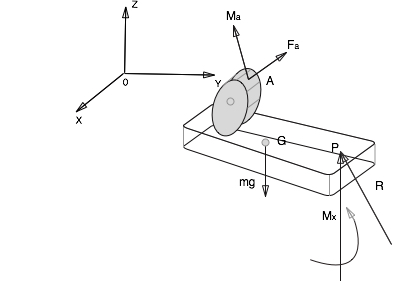
\includegraphics[width=0.5\textwidth]{1}}
		\caption{The sole with acting forces on it}
		\label{fig:1}
		\vspace{-0.1cm}
	\end{figure}

On the figure above we consider the sole without anything upper it. It has its own center of gravity G. At point P there is resulting ground reaction that maintains the construction in the equilibrium. The force of ground reaction R and moment M consists of its three components ($R_x$, $R_y$, $R_z$) and ($M_x$, $M_y$, $M_z$) respectively. Horizontal components of R should compensate friction force in the point of contact. Thus, the horizontal reaction of force ($R_x$, $R_y$) represents 
friction force that compensate horizontal component of $F_a$. In the same time the moment $M_z$ represents friction reaction forces \cref{fig:2} that compensates vertical component of $M_a$ and the moment induced by $F_a$. \cite{vukobratovic2004zero}

	\begin{figure}[h!]
		\vspace{-0.2cm}
		\centering
		{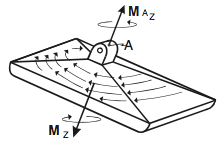
\includegraphics[width=0.5\textwidth]{2}}
		\caption{Rotational moment in the sole}
		\label{fig:2}
		\vspace{-0.1cm}
	\end{figure}

This ZMP should be on the foot. The problem is that we cannot manipulate the foot directly. According to \cite{vukobratovic2004zero} we can do it by ensuring the appropriate dynamics of the mechanism above the foot. If the resulting force in ZMP lies not in vertical direction (conditions from the paragraph above doesn't hold and R and $M_z$ doesn't compensate correspondent components of $F_a$ and $M_a$) than foot will slide. It means that dynamical stability was not achieved due to the fact, that there is a rotational moment that will affect the robot. On the other hand, if ZMP was achieved in the polygon of foot and moreover it coincides with the contact point, than robot is stable, due to the fact, that all the resulting forces lies in vertical direction. During the walk the position of ZMP should be computed simultaneously and the problem of control is to keep ZMP and contact point to be coincided inside the support polygon of contact foot with the ground.
The name zero moment point relates to the fact, that dynamical stability is maintained if horizontal components $M_x$ and $M_y$ are both equal to zero.
	
	\begin{equation}
		M_x = M_y = 0
	\end{equation}

Another words, in the point P there exists such equivalent force R and vertical moment $M_z$ that compensate the ground of force reaction and maintains the stability of the construction. If we want to achieve the dynamical stability, that the following equations holds:

	\begin{equation}
		R + F_a + m_sg = 0
	\end{equation}

Where $m_s$ is a foot mass. In \cite{vukobratovic2004zero} there is defined  point O - the origin coordinates frame from which we can define radius vectors $\vec{OP}$, $\vec{OG}$ and $\vec{OA}$ where A is a point of ankle joint.

	\begin{equation}
		\vec{OP} \times \vec{R} + \vec{OG} \times m_sg + M_A + M_z + \vec{OA} \times F_a = 0
	\end{equation}

Placing the origin frame into the point P and making a projection on the horizontal plane gives us the following equations: 

	\begin{equation}
		(\vec{OP} \times \vec{R})^H + \vec{OG} \times m_sg + M_A^H + (\vec{OA} \times F_a)^H = 0
	\end{equation}

According to \cite{vukobratovic2004zero} equation (4) represents the foot equilibrium. However ot doesn't solve the problem, that it is still unknown whether for the given motion of mechanism it is in the equilibrium. It is only of ZMP lies inside the support polygon.

In \cite{dekker2009zero} it was stated, that we have to make the following assumptions in order to compute the position of ZMP:

	\begin{enumerate}
		\item
			The bipedal robot consists of n rigid links.
		\item
			All kinematic information, such as position of CoM, link orientation, velocities, etc. are known and calculated by forward kinematics.
		\item
			The floor is rigid and motionless.
		\item
			The feet cannot slide over the floor surface.
		\item
			All joints are actively actuated.
	\end{enumerate}
	
With this constraints we can define the mass of the robot as:
	
	\begin{equation}
		m_{robot} = \sum^n_{i=1}{m_i}
	\end{equation}

In \cite{dekker2009zero} it was considered schematic bipedal robot to derive the coordinates of ZMP [Fig. 3]

	\begin{figure}[h!]
		\vspace{-0.2cm}
		\centering
		{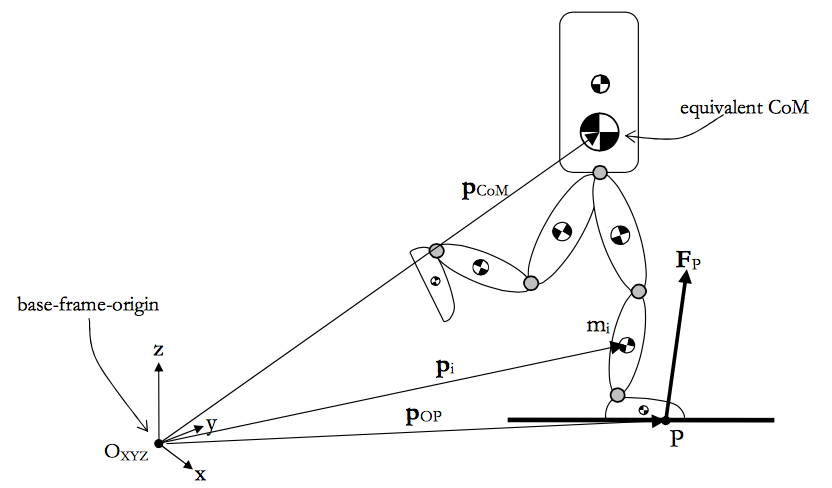
\includegraphics[width=0.5\textwidth]{3}}
		\caption{Rotational moment in the sole}
		\label{fig:3}
		\vspace{-0.1cm}
	\end{figure}

Here $p_i$ are the distances between base frame and equivalent center of mass of i-link. From this total linear momentum P is:
	
	\begin{equation}
		P = \sum^n_{i=1}{m_i \dot{p_i}}
	\end{equation}
And total angular momentum H is:
	\begin{equation}
		H = \sum^n_{i=1}{\dot{p_i} \times m_i \dot{p_i} + I_i \omega_i}
	\end{equation}

Where $\omega_i$ is a angular velocity and $I_i$ is inertia tensor that is computed as:
	\begin{equation}
		I_i = R_i I_i R_i^T
	\end{equation}
Here $R_i$ is a rotation matrix from i-link w.r.t. the origin base frame and $I_i$ is a inertia matrix of i-link w.r.t. the link frame origin attached to their links.

Taking the derivative from 6 and 7 we have got:
	\begin{equation}
		\dot{P} = \sum^n_{i=1}{m_i \ddot{p_i}}
	\end{equation}
	\begin{equation}
		\dot{H} = \sum^n_{i=1}{\ddot{p_i} \times m_i \dot{p_i} + \dot{p_i} \times m_i \ddot{p_i} + I_i \dot{\omega_i}} + \omega_i \times I_i \omega_i
	\end{equation}

In \cite{manchester2011stable} it was mentioned that ZMP approach give us the solution that is based on the principle of dynamical stability, however it is not energy efficient. It requires simultaneous control over all the joints of the robot. The method that was described in \cite{collins2001three} is called passive-walker dynamics and it uses gravity forces to reduce the amount of necessary energy to control the robot.\\
It was mentioned earlier that active control of the robot should be performed with applying dynamical stability principle, elsewhere the robot will loose the balance and fall. So, it makes sense to apply passive-walker dynamics with ZMP based control. According to \cite{vukobratovic2004zero} ZMP method is the most well known and so it is necessary to start with it. Than iteratively increasing the complexity of the problem and applying new technics and constraints we will reach the optimal solution.\\
According to \cite{vukobratovic2004zero} the most important task in the bipedal locomotion is to maintain dynamical stability. It can be accomplished if the foot have a full contact with the ground, it means, that the contact is not only in the edge or in the point. Moreover it shows that ZMP position depends on the robot dynamics: the resulting force in the contact polygon and total moment there. So, during the motion the position of ZMP changes and there are border situations when ZMP reaches the edge of support polygon. In these situations if additional moments appear, robot will rotate around foot edge and collapse. \cite{vukobratovic2004zero} suggests the way to measure the load on the sole via force sensors on it. The algorithm of ZMP control is quite obvious. Compute wanted ZMP coordinates, measure the error and apply correcting signal. Very important notion is about Center of Pressure (CoP). According to \cite{vukobratovic2004zero} the pressure between foot and the ground can be replaced with the force applied in CoP. With this we can define stability condition as ZMP and CoP coincident.\\
In \cite{kim2012zmp} it was mentioned the new approach to solve ZMP control problem. Using neural network trained with back propagation method was used to control the position of the robot given the errors between ZMP position and CoP.
\newpage

\bibliographystyle{unsrt}
\bibliography{robotics}
  
\end{document}

